\documentclass[a4paper]{article}

\usepackage[english]{babel}
\usepackage[utf8x]{inputenc}
\usepackage[framemethod=pstricks]{mdframed}
\usepackage{showexpl}
\usepackage[xindy]{glossaries}
\usepackage{float}

\newcommand{\bgls}[1]{\textbf{\gls{#1}}}
\newcommand{\bglspl}[1]{\textbf{\glspl{#1}}}

\makeglossaries
\newglossaryentry{update transaction}
{
name={Update Transaction},
description={A message signed by both parties, updating the state of a channel. One of the parties posts this to the bank or blockchain to close the channel. However, before this happens an infinite number of \bglspl{update transaction} can be exchanged between the two parties}
}

\newglossaryentry{opening transaction}
{
name={Opening Transaction},
description={A message signed by both parties to create a channel. One of the parties posts this to the bank or blockchain. \bglspl{opening transaction} serve to identify the parties and place funds in escrow}
}

\newglossaryentry{net transfer amount}
{
name={Net Transfer Amount},
description={An amount included in \bglspl{update transaction} which specifies how much money to transfer from \textbf{Party 1} to \textbf{Party 2} when the channel closes. If it is negative, funds are transferred in the other direction}
}

\newglossaryentry{conditional transfer amount}
{
name={Conditional Transfer Amount},
description={An amount included in \bglspl{smart condition} which the bank or blockchain adds to the channel's \bgls{net transfer amount} if one of the parties posts a \bgls{fulfillment} which causes the \bgls{smart condition} to return true}
}

\newglossaryentry{nonce}
{
name={Nonce},
description={An integer included the \bgls{update transaction} which must be incremented with each new \bgls{update transaction}. The bank or the blockchain uses the \bgls{nonce} to ascertain the ordering of \bglspl{update transaction}. An \bgls{update transaction} with a higher \bgls{nonce} will always override one with a lower \bgls{nonce}}
}

\newglossaryentry{hold period}
{
name={Hold Period},
description={A time period included in the \bgls{update transaction}. The bank or blockchain must wait this amount of time before transferring any money when closing the channel. This provides a chance for one of the parties to counteract a cheating attempt where the other party posts an old \bgls{update transaction}. If one of the parties posts a newer \bgls{update transaction} with a higher \bgls{nonce} before the \bgls{hold period} is over, it will override the older \bgls{update transaction}}
}

\newglossaryentry{smart condition}
{
name={Smart Condition},
description={A piece of Turing-complete code included in the \bgls{update transaction} that is evaluated by the bank or blockchain during the \bgls{hold period}. It can return either true or false when supplied with a \bgls{fulfillment}. It has an associated \bgls{conditional transfer amount}, which is added to the channel's \bgls{net transfer amount} if the \bgls{smart condition} returns true}
}

\newglossaryentry{fulfillment}
{
name={Fulfillment},
description={A piece of data used as input to a \bgls{smart condition}. This can be posted at any time during the \bgls{hold period}, and only needs to be signed by one of the parties}
}

\newglossaryentry{payment secret}
{
name={Payment Secret},
description={A secret shared between the source and destination of a multihop payment. The source hahshes the \bgls{payment secret} and gives the hash to the intermediary nodes. Intermediary nodes use it to create \bglspl{hashlock condition} between all the intermediary nodes involved in the multihop payment. The destination reveals the \bgls{payment secret} to the last intermediary node in order to claim the payment. The last intermediary node reveals it to the second-to-last and so on back to the source}
}

\newglossaryentry{hashlock condition}
{
name={Hashlock Condition},
description={A \bgls{smart condition} that hashes its argument, usually a \bgls{payment secret} and compares the hash to a prespecified string. If the hash and the prespecified string match, the \bgls{smart condition} returns true, and the bank or blockchain adds the corresponding \bgls{conditional transfer amount} to the channel's \bgls{net transfer amount}}
}

\newglossaryentry{payment initialization}
{
name={Payment Initialization},
description={A message sent from the source of a multihop payment to the destination, setting up the payment and conveying the \bgls{payment secret} and the \textbf{Amount} of the payment}
}

\newglossaryentry{routing message}
{
name={Routing Message},
description={A message propagated between nodes as part of the routing protocol. It contains the hash of the \bgls{payment secret} and an \textbf{Amount}. Each node that propagates the \bgls{routing message} adds its fee to the \textbf{Amount}}}
}

\newglossaryentry{routing table}
{
name={Routing Table},
description={A table maintained by each node that records \bglspl{routing message} received and forwarded by that node. The node then uses the \bgls{routing table} to route the payment corresponding to a given \bglspl{routing message}}
}

\mdfdefinestyle{message}
{
  nobreak=true,
  leftmargin=10,
  rightmargin=10,
  innerleftmargin=20,
  innerrightmargin=20,
  innertopmargin=10,
  innerbottommargin=10,
  skipabove=20pt,
  skipbelow=20pt
}

\setlength{\parskip}{3pt}

\newenvironment{mydescription}
{\begin{description}
\setlength{\itemsep}{5pt}
  \setlength{\parskip}{0pt}
  \setlength{\labelsep}{5pt}
}{
\end{description}}

\title{Reactive Payment Routing}
\author{Jehan Tremback\\
\texttt{jehan.tremback@gmail.com}\\}
\date{November 2015\\
\texttt{v0.4}}

\begin{document}
\maketitle

\begin{abstract}
\end{abstract}

\section{Routing multihop payments}

If you're going to have a multihop payment network, you need some way to route payments. How does Alice know that sending a payment through Bob will be the cheapest way to reach Charlie? Perhaps Benjamin also has channels open with Alice and Charlie but he charges a lower fee. There needs to be some way to find the lowest-priced route to a payment's destination. This problem resembles the problem of routing packets on the internet, so we will look at some possible solutions from that domain.

One can separate ad-hoc routing protocols into two main categories--- proactive and reactive. Proactive protocols work by exchanging messages to build up routing tables listing the next hop for each address on the network. When a node receives a packet, it can immediately forward the packet along to the best peer to get it closer to its destination. However, every node needs to have an entry in its routing table for every other node. On a large network, this becomes infeasible.

In reactive protocols, nodes request a route from the network when they need to send packets to a new destination. This means that nodes don't need to store information on every single destination, and connectivity changes do not result in the update of every node's routing tables. However, the initial route discovery process adds some unavoidable latency when sending to new destinations.

For most payments, a few hundred milliseconds to establish a route does not present a problem. Needing to store a routing table entry for every address in the network is far worse. For this reason we'll use a variation of Ad hoc On-Demand Distance Vector Routing (AODV) \cite{aodv}, a reactive routing protocol.

In AODV, when nodes need to send a packet to a destination they have never sent a packet to, they send out a \textbf{Route Request Message}, which is flooded through the network (with some optimizations). When the destination receives this message, it sends a \textbf{Route Reply Message}. Intermediary nodes along the path cache the next hops for the source and the destination, thereby storing only the routing information they are likely to need often.

\subsection{Reactive Payment Routing}

Since our nodes are presumed to already have internet connectivity, we can skip the \textbf{Route Request Message}. Our protocol has only one type of message, which we'll call the \bgls{routing message}. A node's neighbors are those nodes that it has payment channels open with.

When a node (which we'll refer to as the source) wishes to send a multihop payment, it first sends a \textbf{Payment Initialization} to the destination of the payment.

\begin{mdframed}[style=message]{\emph{Source to destination}}
\begin{mydescription}
\item[Payment Initialization:] \hfill
\begin{mydescription}
  \item[Secret:] Payment secret.
  \item[Amount:] Amount of payment.
\end{mydescription}
\end{mydescription}
\end{mdframed}

The destination then constructs a \bgls{routing message}. The routing message includes the hash of the payment secret, and the amount of the payment. It sends the \bgls{routing message} to all of its neighbors who have enough in their channels to cover the payment (if Dolores wants to receive \$100, she won't send the \bgls{routing message} to Clark, who only has \$20 in his side of the channel).

\begin{mdframed}[style=message]{\emph{Destination to neighbors}}
\begin{mydescription}
\item[Routing Message:] \hfill
\begin{mydescription}
  \item[Hash:] Hash of payment secret.
  \item[Amount:] Amount of payment.
\end{mydescription}
\end{mydescription}
\end{mdframed}

When a node receives a \bgls{routing message}, the node makes a new \textbf{Routing Table Entry}.

\begin{mdframed}[style=message]{\emph{Saved in routing table}}
\begin{mydescription}
\item[Routing Table Entry:] \hfill
\begin{mydescription}
  \item[Hash:] Hash of payment secret.
  \item[Amount:] Amount of payment.
  \item[Neighbor:] The neighbor that the \bgls{routing message} came from.
\end{mydescription}
\end{mydescription}
\end{mdframed}

The node also sends the \bgls{routing message} along to neighbors with enough to cover the payment, but not before adjusting the \textbf{Amount}. To adjust the \textbf{Amount}, the node adds the fee that it would like to receive for routing the payment. Also, if the node is sending the \bgls{routing message} to a neighbor with whom it has a channel open in a different currency, the \textbf{Amount} is converted to that currency.

\begin{mdframed}[style=message]
\begin{mydescription}
\item[Routing Message:] \hfill
\begin{mydescription}
  \item[Hash:] Hash of payment secret.
  \item[Amount:]   $(payment + fee) * exchange\_rate$
\end{mydescription}
\end{mydescription}
\end{mdframed}

The \bgls{routing message} can be thought of as asking one implicit question: ``How much would someone have to send you for you to send me \textbf{Amount}?'' By adjusting the amount, a node is informing the network how much it charges to transfer money, and consequently, how good the route that it is on is. The \textbf{Routing Table Entry} makes sure the node routes the actual payment correctly, if it is on the winning route.

If a node receives a \bgls{routing message} with the same \bgls{payment secret} hash again, it will compare the \textbf{Amount} of the new \bgls{routing message} with the \textbf{Amount} that it has stored in its \bgls{routing table}. If the \textbf{Amount} of the new \bgls{routing message} is lower than what is in the \bgls{routing table}, it will update the \bgls{routing table} and send out a new \bgls{routing message}.

The \bglspl{routing message} propagate until they reach the source of the payment. At this point, the source can continue to wait, because it may receive another \bgls{routing message} with a lower \textbf{Amount}. If the source is satisfied with the \textbf{Amount}, it then uses the \bgls{payment secret} hash to make a hashlocked payment to the neighbor that sent it the routing message. This neighbor then checks their routing table and makes a payment to their corresponding neighbor. The hashlocked payments continue until they reach the destination, at which point it unlocks the payment with the secret, letting the rest of the chain unlock their payments as well (as explained in ``Multiphop Channels'' above).

\pagebreak

\begin{figure}[H]
\centering
\makebox[\textwidth][c]{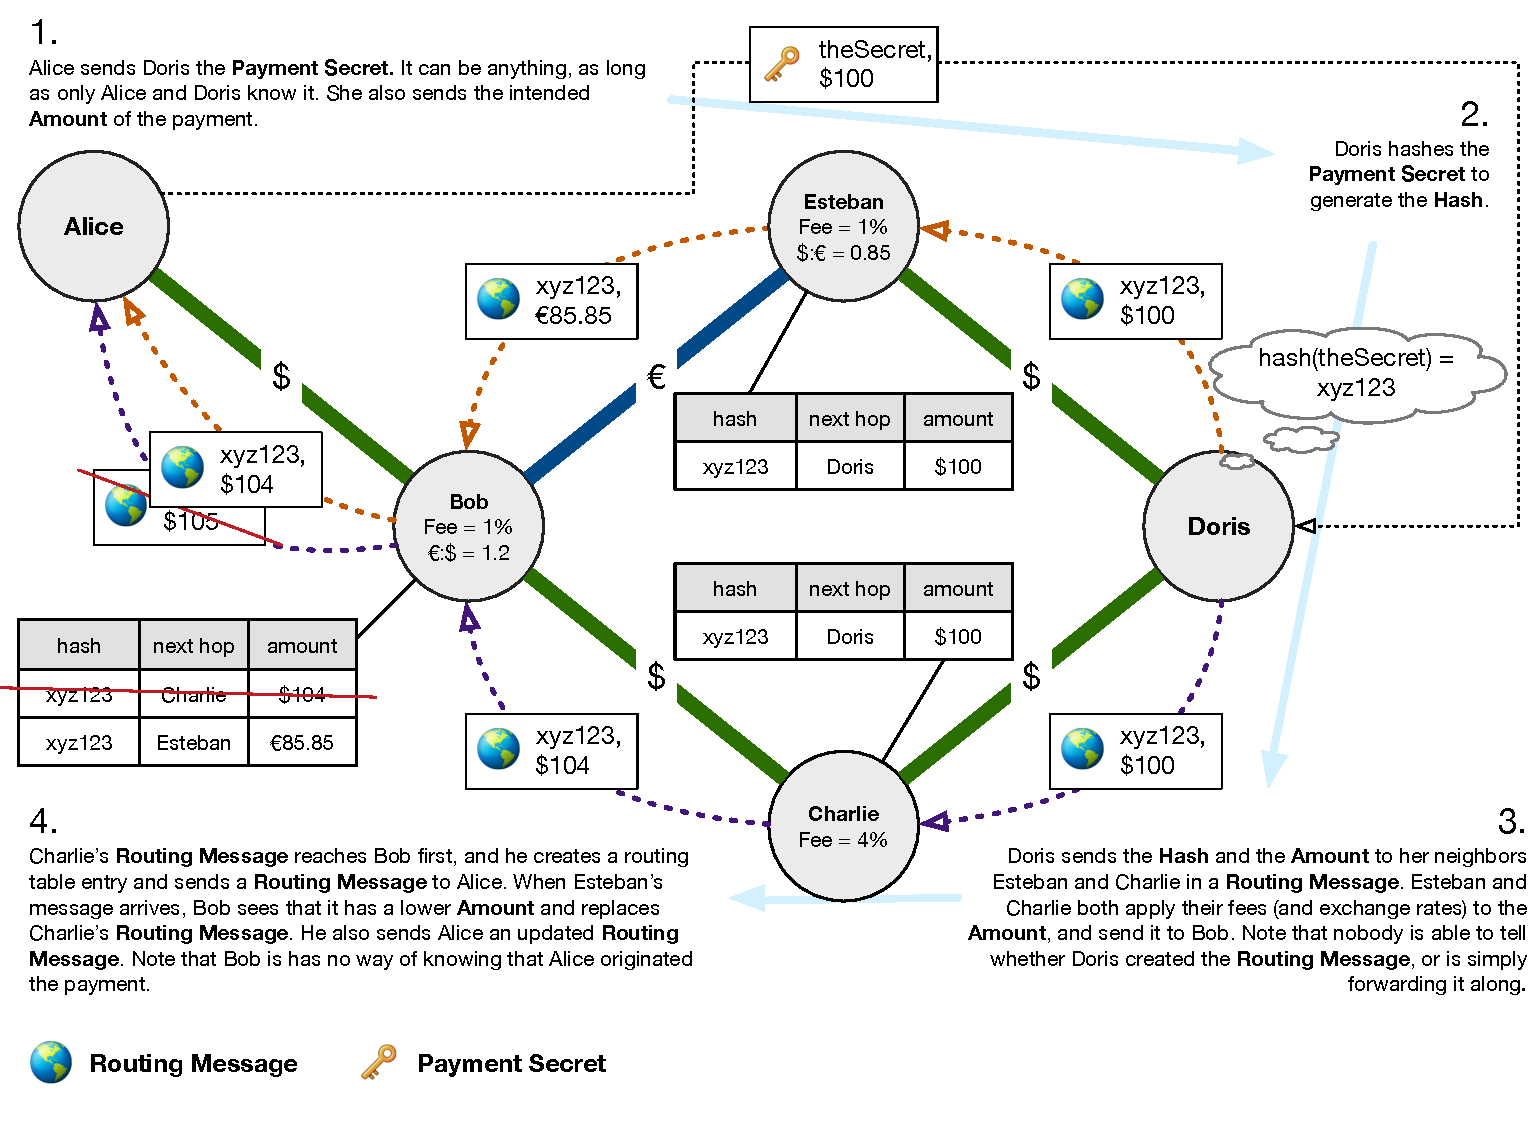
\includegraphics[width=1.5\textwidth]{routing.pdf}}
\caption{Finding a payment route}
\end{figure}

\begin{figure}[H]
\centering
\makebox[\textwidth][c]{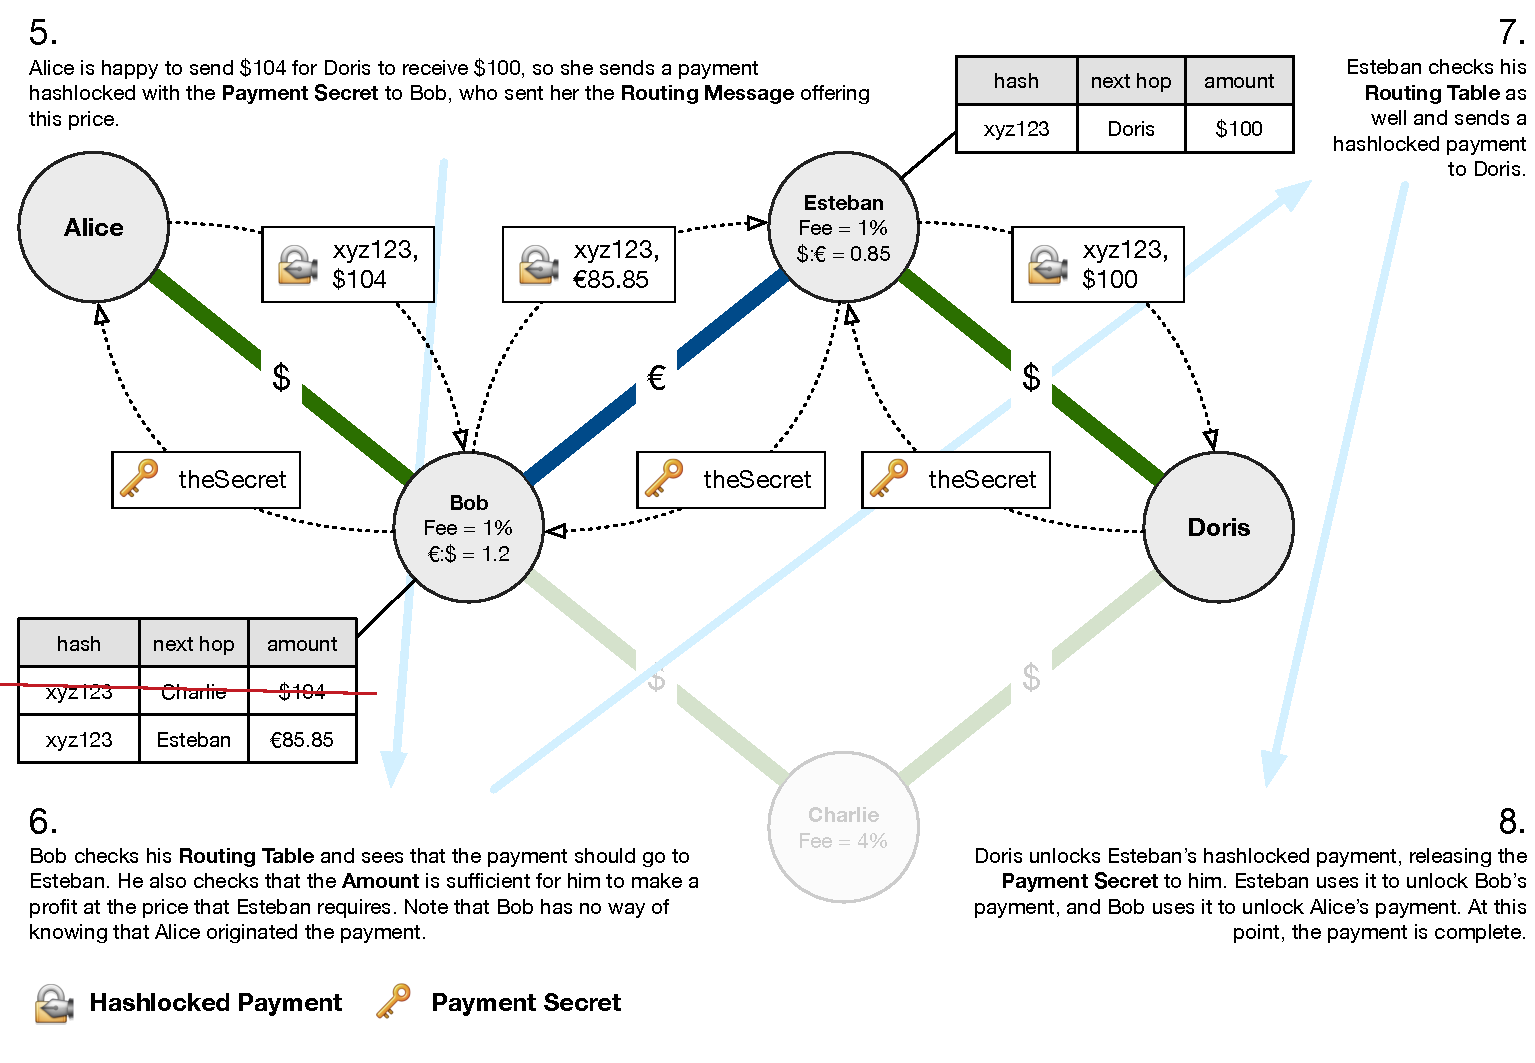
\includegraphics[width=1.5\textwidth]{payment.pdf}}
\caption{Sending a hashlocked payment along a route}
\end{figure}

\pagebreak

\printglossaries

\begin{thebibliography}{99}

\bibitem{interledger}
\emph{A Protocol for Interledger Payments}\\
Stephan Thomas, Evan Schwartz\\
\texttt{https://interledger.org/interledger.pdf}\\
2015

\bibitem{btcwiki}
\emph{Micropayment Channel}\\
Bitcoin Wiki Contributors\\
\texttt{https://bitcoin.org/en/developer-guide\#micropayment-channel}\\
2014

\bibitem{bitcoinj}
\emph{[ANNOUNCE] Micro-payment channels implementation now in bitcoinj}\\
Mike Hearn\\
\texttt{https://bitcointalk.org/index.php?topic=244656.0}\\
2013

\bibitem{blueadept}
\emph{Decentralized networks for instant, off-chain payments}\\
Alex Akselrod\\
\texttt{https://en.bitcoin.it/wiki/User:Aakselrod/Draft}\\
2013

\bibitem{amiko}
\emph{Amiko Pay}\\
C. J. Plooy\\
\texttt{http://cornwarecjp.github.io/amiko-pay/doc/amiko\_draft\_2.pdf}\\
2013

\bibitem{duplexchannels}
\emph{A Fast and Scalable Payment Network with Bitcoin Duplex Micropayment Channels}\\
Christian Decker, Roger Wattenhofer\\
\texttt{http://www.tik.ee.ethz.ch/file/716b955c130e6c703fac336ea17b1670/\\duplex-micropayment-channels.pdf}\\
2015

\bibitem{lightning}
\emph{The Bitcoin Lightning Network: Scalable Off-Chain Instant Payments}\\
Joseph Poon, Thaddeus Dryja\\
\texttt{https://lightning.network/lightning-network-paper.pdf}\\
2015

\bibitem{aodv}
\emph{Ad-hoc On-Demand Distance Vector Routing}\\
Charles E. Perkins, Elizabeth M. Royer\\
\texttt{https://www.cs.cornell.edu/people/egs/615/aodv.pdf}\\

\bibitem{ethereum}
\emph{A Next-Generation Smart Contract and Decentralized Application Platform}\\
Vitalik Buterin\\
\texttt{https://github.com/ethereum/wiki/wiki/White-Paper}\\
2014

\bibitem{tendermint}
\emph{Tendermint: Consensus without Mining}\\
Jae Kwon\\
\texttt{http://tendermint.com/docs/tendermint.pdf}\\
2015

\bibitem{flyingfox}
\emph{Flying Fox}\\
Zackary Hess\\
\texttt{https://github.com/BumblebeeBat/FlyingFox}\\
2015

\end{thebibliography}

\end{document}